
\documentclass[11pt, letterpaper]{article}
%\usepackage{bookmark}
\usepackage[a4paper,margin=2cm]{geometry}
\usepackage[]{graphicx}
\usepackage{bm}
\usepackage[strings]{underscore}
\usepackage{apacite}
\setlength{\parindent}{0pt}
\graphicspath{ {./Images} }
\usepackage{wrapfig}
\begin{document}
\begin{titlepage}
	\title{Modelling and Lighting Interior Spaces using Reflected Natural Light}
	\author{Noah Alexiou}
	\date{\today}
	
	\maketitle
	\centering
	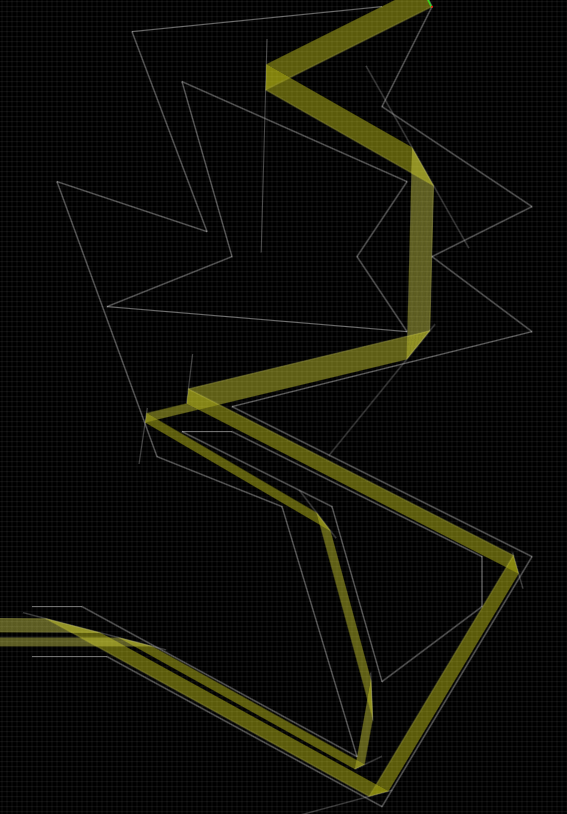
\includegraphics[width=14cm]{cave2.png}
	
\end{titlepage}

\newpage
\tableofcontents


\newpage

\section{Introduction}


\subsection{Premise}
This study aimed to find optimal mirror placement for minimum decrease in intensity as light travelled throughout a given cave. This was achieved by mapping the cave's geometry and simulating the possible paths of light as a vector throughout the cave with various mirror arrangements.




\subsection{Assumptions} 
\par

In Order for an accurate solution to be formed, a set of conditions had to be assumed in order to simplify modelling and remove ambiguity.
\begin{itemize}

	\item The given specifications did not provide an orientation, so it was assumed that the cave described was traversed horizontally and depicted 'top-down'.
	
	\item Mirrors and walls of the cave were parallel to the floor and extended upwards with an undefined height. Light entered the cave parallel to the ground with uniform intensity. This simplified modelling and could easily be altered if height was defined. 
	

	\item Either light did not decrease in intensity or increase in area according to the inverse square law, or the change was negligible. The suns rays have travelled so far that they can be considered effectively parallel and therefore did not diverge. 
	\cite{yasuda_2024_why}
		
	\item Mirrors reflected light across their entire surface. Light only intersected a mirror and reflected across the normal or did not intersect with a mirror at all. This meant that only mirror surfaces had to be accounted for
	
	\item Mirrors were perfectly flat and did not distort or affect light beams in any other way than reflecting them. While unrealistic to expect in the real world, such factors are out of the scope of this study.
	
	\item While the entry and exit vectors had no width, it was assumed that light entered the cave through the entire entrance, and could exit throughout the entire exit. Each point along the entrance was considered the beginning of its own vector, with equal direction to the entry vector.  This allowed the entire beams width to be accounted for without introducing unnecessary calculations. 
	
	\item The stimulus implies that the light entering the cave was from the sun, however the sun's position in the sky is constantly changing. Therefore it was assumed that the entry vector's was constant.
		


\end{itemize}

\subsection{Observations}
\par

The following observations were made and their impacts on the solution's success criteria, or working were evaluated.
\begin{itemize}




\item Contaminants in the air may decrease the intensity of light. Distance light travels in cave must be minimised to avoid loss in intensity.

\item Mirrors are imperfect and will only reflect a portion of light that hits them.  Therefore the number of mirrors used must also be minimised to avoid loss in intensity.

\item Only the edges of each beam of light needed to be found as any light that is within a beam was travelling the same direction as the light at the edges. This allowed intersections with mirrors and cave walls to be found without introducing unnecessary calculations.

\item Clearly paths were not wide enough for a beam of 2 units, the size of the cave's entrance, to pass through them. Therefore the beam was required to be split in order for light to be passed through the cave efficiently.

\item In the case of the beam being split, the edges of each beam were found and each considered the new edge for the split path.
\newline
\begin{center}
\includegraphics[width = 12cm]{new diagram.jpg}

{Figure 1: Expected and assumed behaviour when beam is split}
\end{center}
\end{itemize}





\subsection{Translation}
\par 



Light can be modelled as a relative position vector with origin at a mirror surface on the Cartesian plane and translated without affecting its other properties. When a reflection occurs, $\textrm{angle  of incidence} = \textrm{angle of refraction}$.
 
The scalar product between 2 vectors is a measure of how closely a set of two vectors match each others direction. To find the scalar product, the equation $\textbf{a }\cdot \textbf{b}=|\textbf{a}|\cdot|\textbf{b}| \cdot \textrm{cos}(\theta)$ was used. Clearly for this application, $a$ and $b$ would be listed in traditional component form, When rearranged as $\textrm{cos}^{-1}{(\frac{x_1 \cdot x_2 + y_1 \cdot y_2}{|\textbf{a}|\cdot|\textbf{b}|})} = \theta$ the acute angle between 2 vectors, when arranged tail-to-tail, could be found
\newline
Tools such as desmos mapped vectors as an arrows that span 2 points. The $x$ and $y$ values that usually refer to a direction and magnitude were converted into 2 discrete sets points, in which one defines the starting point of a vector, and one defines the end. It must be noted that unless explicitly stated, the latter format is what is being used to describe vector position, not regular component form.
\par

The proportion of light remaining after $n$ number of reflections was modelled as the exponential $I=\textrm{Efficiency}^x$, where $I$ is a scalar representation of intensity with respect to the original intensity , $n$ is the number of mirrors, and $\textrm{Efficiency}$ is the percentage  efficiency of the mirror in decimal form. Clearly, adding more mirrors will lead to diminishing losses in intensity.
\newline
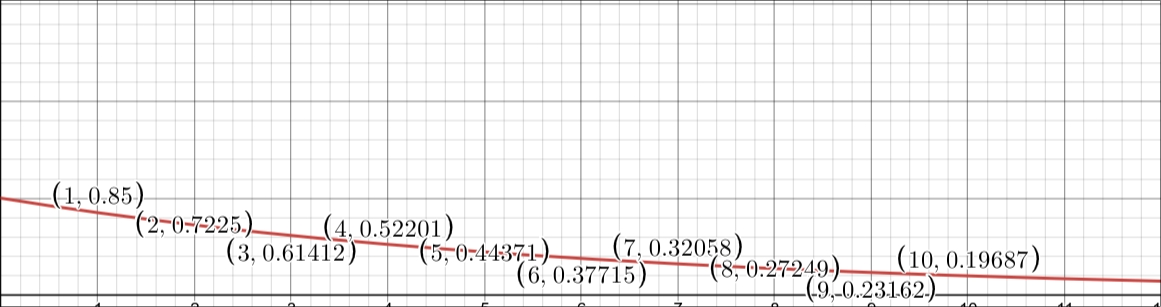
\includegraphics[width=16cm]{Diagram 7.jpg}
\begin{center}
{Figure 2: The exponential $0.85^x$ showing number of mirrors on $x$-axis, and scalar intensity on $y$-axis}
\end{center}



\par 


\section{Solve}

\par 


To map out the cave and its obstacles, the list of conjoined vectors had to be converted into Cartesian co-ordinates. This was achieved through considering the vector sum of the first $n_{th}$ vectors that made up an object as tail of a new vector, then doing the same with the  $(n+1)_{th}$ vector sum, and considering it the head. This gave the relative position vector of the new wall. These calculations were completed in Excel with vectors in component form. \newline
The co-ordinates of the start and end points of the left wall were arranged into a chain of interconnected $x$, and $y$ co-ordinates and inserted into desmos as lists $X_1$, and $Y_1$ respectively. These lists were then plotted as connected points. The same was repeated for the remaining wall, and obstacle geometry.

These lists were also manually inserted into the phydemo.app light ray simulator using the text based editor. When the lists were initially imported the scale was imperceptibly small and the $y$-axis was inverted. To solve this, all points had their $x$ components scaled by a factor of 100, and their $y$ components by a factor of -100. Henceforth any mention of points in the context of the phydemo.app simulator will be in reference to these scaled points.
\newline
In the phydemo simulator, light is emitted from the normal of objects. Therefore the entry vector was required to be rotated by $90^\circ$ by swapping its $\textbf{i}$ and $\textbf{j}$ components, then multiplying the new j component by -1. It was then offset so that its tail was positioned at the edge of the cave's right entrance, at $(16, 0)$, and plotted at a relative position vector, by adding its components to the co-ordinates of its tail. It was found that the width of its emitted beam matched that of the width of the entrance. No further intervention was required. 
\newline
\begin{wrapfigure}{l}{0.24 \textwidth}
		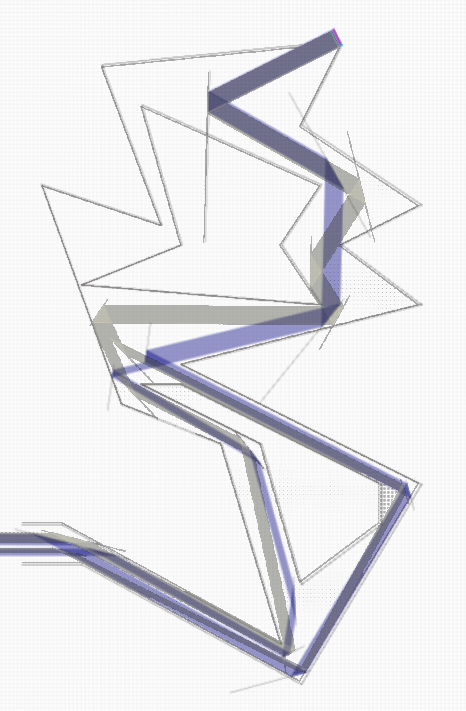
\includegraphics[width=0.24\textwidth]{Diagram 8.png}
	\begin{center}

{Figure 3: A comparison of an early (black) and final (purple) path iterations}
	\end{center}
\end{wrapfigure}

Once the entry vector was positioned, mirrors were manually placed and adjusted so that light travelled throughout the cave and exited parallel. Then began an iterative process with the goal of (in order of priority) reducing light absorbed into the cave walls/resolving collisions, decreasing reflections that the light underwent before exiting, and/or reducing the distance that light had to travel before exiting. 


The initial drafted solution required light to undergo 9 reflections in order to reach the exit. This was reduced to 7 in the final revision. The differences between these solutions were the removal of a mirror beside the first obstacle,and a mirror directly before the beam was split. These changes not only reduced the number of mirrors required, but the distance that the beam travelled. No solutions that did not split the beam of light were considered as intentionally losing light was counter intuitive to the task.


Once a satisfactory mirror arrangement was achieved, the start and end points of each mirror were extracted from the phydemo.app simulator and converted back into Cartesian co-ordinates and inserted into desmos as separate lists so the $n_{th}$ element of each list corresponded to the $x$ or $y$ co-ordinate, of either the start or and of the $n_{th}$ mirror. These lists were defined as $x_1$, $y_1$, $x_2$, and $y_2$.

 By defining a vector from the $n_{th}$ element of each corresponding list, the mirrors could be depicted in desmos. The same was done but with the 'line' function, rather than the 'vector' function, as to create an object compatible with desmos's intersection and angle measurement tools.

For each entry vector (originating from the left and right sides of the cave's entrance), the path of the incoming beam of light to the mirror was found and defined as a new vector with components $(x_2 - x_1)\textbf{i}$ and $(y_2 - y_1)\textbf{j}$. This value was used to find the acute angle between the incoming ray, and the mirror $(\theta _1$). The angle between the mirror and the negative $x\textrm{-axis}$ $(\theta _2)$ was also found.
\pagebreak
\newline
\begin{wrapfigure}{l}{0.57 \textwidth}
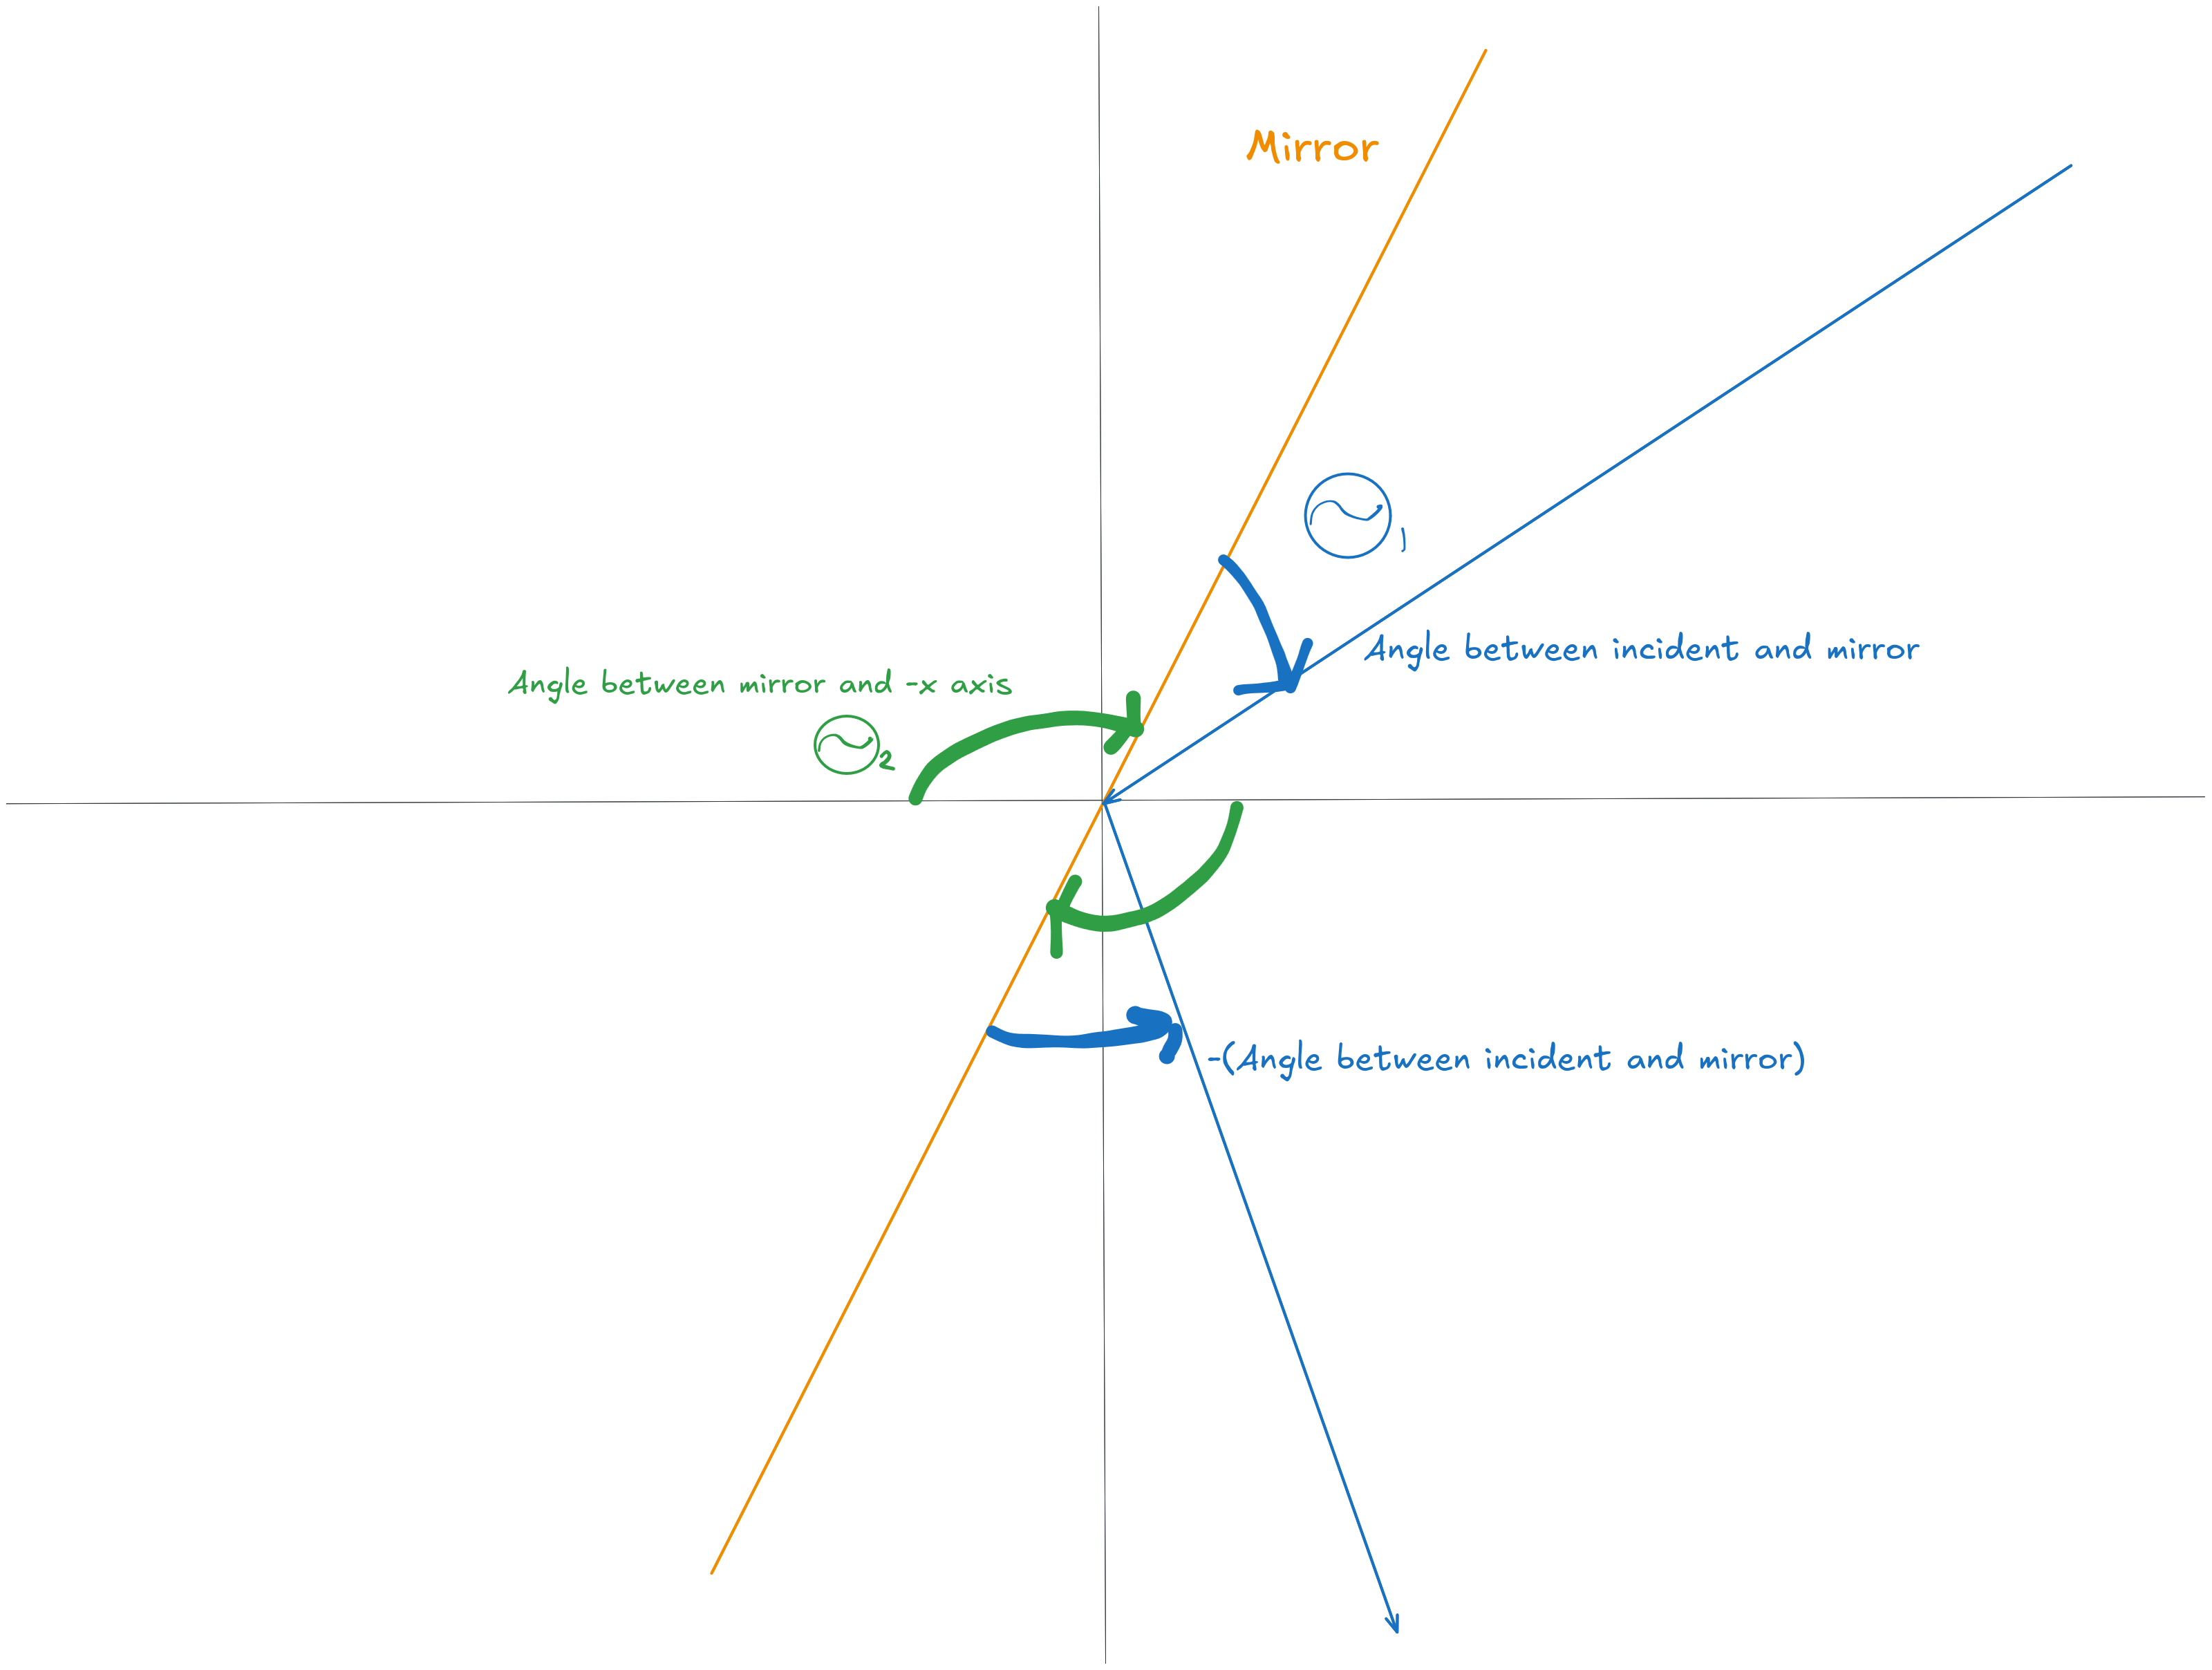
\includegraphics[width=10cm]{Diagram 6.png}
Figure 4: A diagram showing how $\theta _1$ and $\theta _2$ are used to find the angle of the reflected beam.
\end{wrapfigure}


By performing the operation $- \theta_2 + \theta_1 $, the angle of the new beam could be found. This line was then plotted in polar form with infinite magnitude.
This process was repeated for remaining reflections across all paths until the angle of the exiting beam could be found. Mirror positions were redefined so that they started and ended at the points in which their respective beams intersected with them so that they were as small as physically possible. This change was implemented in Excel, however, diagrams and depictions were not updated.




\section{Evaluate and Verify}

To verify that the solution was valid, all light vectors were visually inspected for unintended collisions in desmos. Comparing the intended exit vector to the actual exit vectors showed that the ray of light to the left of the second obstacle, exited at $-180.140271880705^{\circ}$, while the other exited at $-180.001018112731	^\circ$. This was considered acceptable as both values were within $0.15^\circ$ of the intended exit vector: $-180^\circ$.

If the efficiency of each mirror was considered $85\%$, the intensity after 7 reflections would have been $0.85^7 \approx 0.32$. This was considered acceptable as it was $\approx 9\%$ better than initial solutions and the direction of further optimisation was unclear.


\subsection{Strengths and Limitations of Solution}
\subsubsection{Strengths}
\begin{itemize}
\item No light was lost through absorption into the cave walls as beam was able to be split. Clearly this had a large impact on the quantity of exiting light.
\item Light entering throughout the entire entrance was considered and reflected to the exit as opposed to a single vector or light ray.

\item Multiple iterations show direct improvement in solution.

\end{itemize}
\subsubsection{Limitations}
\begin{itemize}
\item Beams never come together as they were at the entrance, and exit at incorrect angles. 

\item Low tolerance for error in mirror placement in case of physical installation, which is imminent considering the context of the task

\item No investigation into alternative methods of directing light, such as curved mirrors, lenses, or beam expansion/compression.

\item Solution not easily optimisable nor mathematically proven to be the best. The process of synthesising new light paths is not automated nor easily optimisable therefore to iterate on the solution, a significant amount of manual intervention is required

\end{itemize}
\section{Conclusion}
The given solution provided a valid mirror arrangement that successfully reflected light through the cave while minimising losses and utilising multiple alternative routes. 

 \section{Appendices}
 
\begin{center}

\begin{tabular}{|c|c|c|c|c|c|c|}
	\hline
	Object & x1 & y1 & neg y1 & x2 & y2 & neg y2 \\
	\hline
	Mirror 1 & 9.37239 & -2.3138 & 2.3138 & 9.34481 & -3.32759 & 3.32759 \\
	\hline
	Mirror 2 & 15.20404 & -5.63765 & 5.63765 & 16.05624 & -7.1486 & 7.1486 \\
	\hline
	Mirror 3 & 15.90875 & -12.97034 & 12.97034 & 14.98217 & -14.11637 & 14.11637 \\
	\hline
	Mirror 4 & 6.25553 & -15.30591 & 15.30591 & 6.188 & -15.872 & 15.872 \\
	\hline
	Mirror 5 & 4.58262 & -16.25859 & 16.25859 & 4.52708 & -16.63408 & 16.63408 \\
	\hline
	Mirror 6 & 11.3956 & -20.26068 & 20.26068 & 11.96353 & -21.00241 & 21.00241 \\
	\hline
	Mirror 7 & 19.26916 & -21.99586 & 21.99586 & 19.47144 & -22.70065 & 22.70065 \\
	\hline
	Mirror 8 & 13.58552 & -26.89374 & 26.89374 & 13.67728 & -28.54813 & 28.54813 \\
	\hline
	Mirror 9 & 13.58371 & -31.5464 & 31.5464 & 14.31294 & -31.36601 & 31.36601 \\
	\hline
	Mirror 10 & 1.063757 & -24.61176 & 24.61176 & 3.34964 & -25.20674 & 25.20674 \\
	\hline
	Mirror 11 & 13.01008 & -30.63217 & 30.63217 & 13.38482 & -30.44808 & 30.44808 \\
	\hline
	
\end{tabular}

{Appendix 1: A table showing the final, trimmed positions of each mirror}
\end{center}
\begin{center}

\begin{tabular}{|c|c|c|c|c|c|c|}
	\hline
	Object Type & x1 & y1 & neg y1 & x2 & y2 & neg y2 \\
	\hline
	Mirror 1 & 9.4 & 1.299 & -1.299 & 9.168 & 9.827 & -9.827 \\
	\hline
	Mirror 2 & 17.471 & 9.657 & -9.657 & 13.365 & 2.377 & -2.377 \\
	\hline
	Mirror 3 & 16.116 & 12.714 & -12.714 & 11.877 & 17.957 & -17.957 \\
	\hline
	Mirror 4 & 6.423 & 13.902 & -13.902 & 6.188 & 15.872 & -15.872 \\
	\hline
	Mirror 5 & 4.283 & 18.284 & -18.284 & 4.612 & 16.06 & -16.06 \\
	\hline
	Mirror 6 & 12.16 & 21.259 & -21.259 & 10.696 & 19.347 & -19.347 \\
	\hline
	Mirror 7 & 19.225 & 21.842 & -21.842 & 19.636 & 23.274 & -23.274 \\
	\hline
	Mirror 8 & 13.572 & 26.65 & -26.65 & 13.705 & 29.048 & -29.048 \\
	\hline
	Mirror 9 & 10.411 & 32.423 & -32.423 & 14.41 & 31.342 & -31.342 \\
	\hline
	Mirror 10 & 5.36 & 25.73 & -25.73 & -0.353 & 24.243 & -24.243 \\
	\hline
	Mirror 11 & 12.986 & 30.644 & -30.644 & 14.138 & 30.083 & -30.083 \\
	\hline
\end{tabular}
\end{center}
\begin{center}
{Appendix 2: A table showing raw imported values of each mirror}
\end{center}




\begin{center}
\includegraphics[width=0.7\linewidth]{../../../../../../../../Pictures/2024-11-24-233025_hyprshot}

\end{center}
\begin{center}
{Appendix 3: A screenshot of the desmos environment with final mirror placements}
\end{center}

\begin{center}
	\includegraphics[width=0.7\linewidth]{../../../../../../../../Pictures/2024-11-24-233035_hyprshot.png}
	
\end{center}
\begin{center}
{Appendix 4: A screenshot of the desmos environment with final mirror placements and connecting lines}
\end{center}

\begin{center}
	\includegraphics[width=0.7\linewidth]{../../../../../../../../Pictures/2024-11-24-234059_hyprshot.png}
	
\end{center}
\begin{center}
{Appendix 5: The provided stimulus}
\end{center}

 \bibliographystyle{apacite}
 \bibliography{References}

\end{document}
